\documentclass{standalone}
\usepackage{tikz}
\usetikzlibrary{patterns, positioning}


\begin{document}
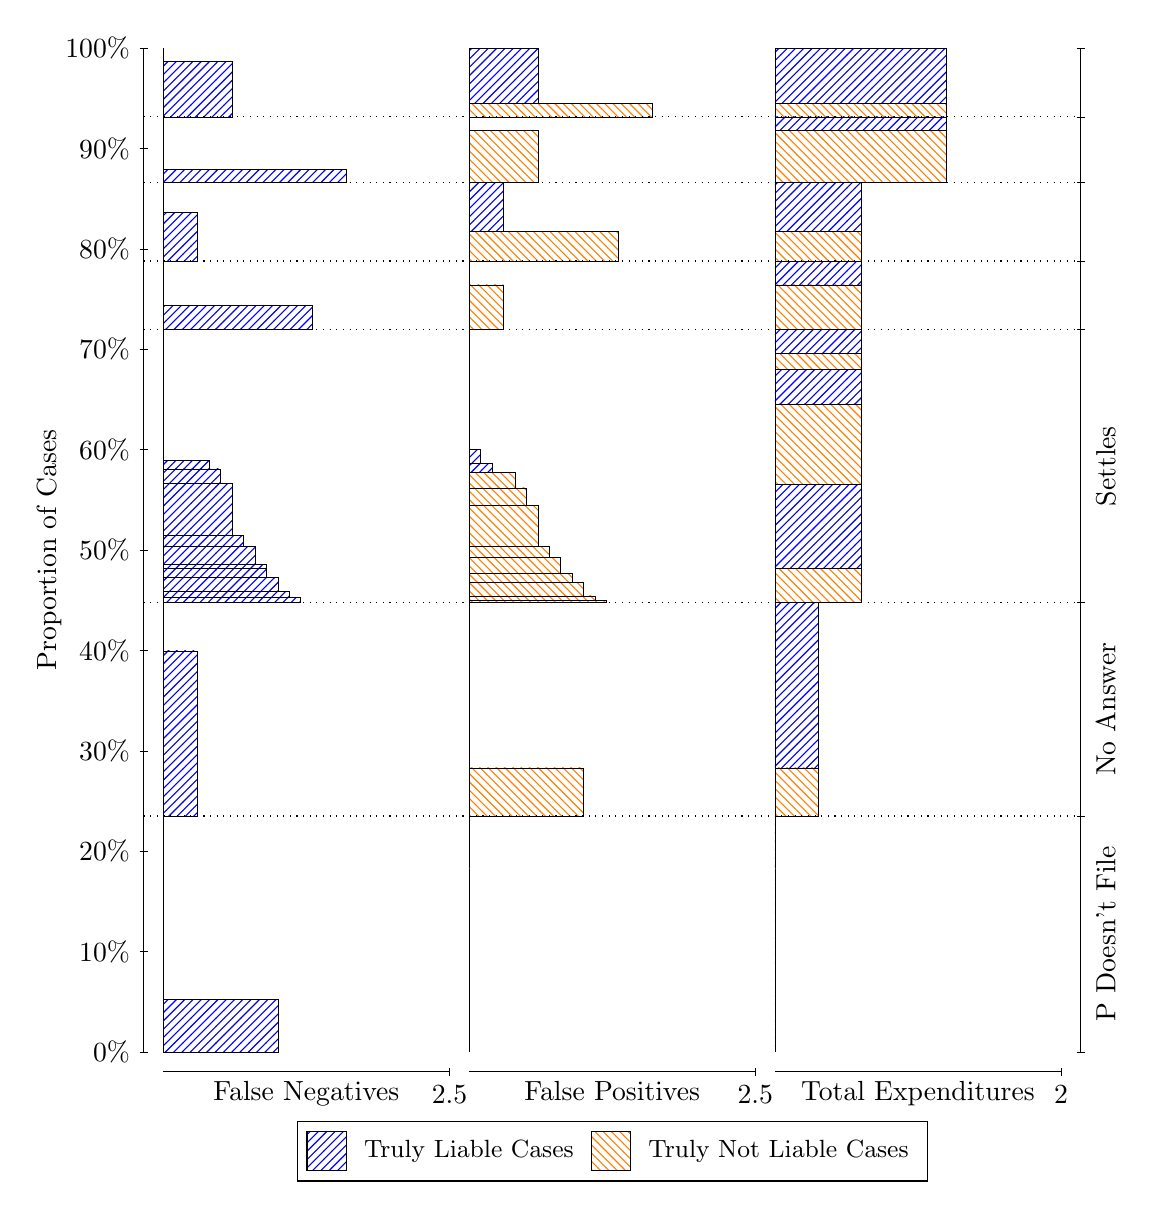
\begin{tikzpicture}
\draw[black, very thin] (1.5,1.75) -- (1.5,14.5);
\node[rotate=90, text=black, anchor=center] at (0.3, 8.125) {Proportion of Cases};
\draw[black, very thin] (1.45,1.75) -- (1.55,1.75);
\node[text=black, anchor=east] at (1.45, 1.75) {0\%};
\draw[black, very thin] (1.45,3.025) -- (1.55,3.025);
\node[text=black, anchor=east] at (1.45, 3.025) {10\%};
\draw[black, very thin] (1.45,4.3) -- (1.55,4.3);
\node[text=black, anchor=east] at (1.45, 4.3) {20\%};
\draw[black, very thin] (1.45,5.575) -- (1.55,5.575);
\node[text=black, anchor=east] at (1.45, 5.575) {30\%};
\draw[black, very thin] (1.45,6.85) -- (1.55,6.85);
\node[text=black, anchor=east] at (1.45, 6.85) {40\%};
\draw[black, very thin] (1.45,8.125) -- (1.55,8.125);
\node[text=black, anchor=east] at (1.45, 8.125) {50\%};
\draw[black, very thin] (1.45,9.4) -- (1.55,9.4);
\node[text=black, anchor=east] at (1.45, 9.4) {60\%};
\draw[black, very thin] (1.45,10.675) -- (1.55,10.675);
\node[text=black, anchor=east] at (1.45, 10.675) {70\%};
\draw[black, very thin] (1.45,11.95) -- (1.55,11.95);
\node[text=black, anchor=east] at (1.45, 11.95) {80\%};
\draw[black, very thin] (1.45,13.225) -- (1.55,13.225);
\node[text=black, anchor=east] at (1.45, 13.225) {90\%};
\draw[black, very thin] (1.45,14.5) -- (1.55,14.5);
\node[text=black, anchor=east] at (1.45, 14.5) {100\%};

\draw[black, very thin] (13.4,1.75) -- (13.4,14.5);
\draw[black, very thin] (13.35,1.75) -- (13.45,1.75);
\node[anchor=west] at (13.35, 1.75) {};
\draw[black, very thin] (13.35,4.7467) -- (13.45,4.7467);
\node[anchor=west] at (13.35, 4.7467) {};
\draw[black, very thin] (13.35,7.4568) -- (13.45,7.4568);
\node[anchor=west] at (13.35, 7.4568) {};
\draw[black, very thin] (13.35,10.923) -- (13.45,10.923);
\node[anchor=west] at (13.35, 10.923) {};
\draw[black, very thin] (13.35,11.795) -- (13.45,11.795);
\node[anchor=west] at (13.35, 11.795) {};
\draw[black, very thin] (13.35,12.79) -- (13.45,12.79);
\node[anchor=west] at (13.35, 12.79) {};
\draw[black, very thin] (13.35,13.625) -- (13.45,13.625);
\node[anchor=west] at (13.35, 13.625) {};
\draw[black, very thin] (13.35,14.5) -- (13.45,14.5);
\node[anchor=west] at (13.35, 14.5) {};

\draw[black, very thin, pattern color=blue, pattern=north east lines] (1.75,1.75) rectangle (3.2033,2.4166);
\draw[black, very thin, pattern color=orange, pattern=north west lines] (1.75,2.4166) rectangle (1.75,4.7467);
\draw[black, very thin, pattern color=blue, pattern=north east lines] (1.75,4.7467) rectangle (2.186,6.8451);
\draw[black, very thin, pattern color=orange, pattern=north west lines] (1.75,6.8451) rectangle (1.75,7.4568);
\draw[black, very thin, pattern color=blue, pattern=north east lines] (1.75,7.4568) rectangle (3.494,7.5225);
\draw[black, very thin, pattern color=blue, pattern=north east lines] (1.75,7.5225) rectangle (3.3487,7.6036);
\draw[black, very thin, pattern color=blue, pattern=north east lines] (1.75,7.6036) rectangle (3.2033,7.7779);
\draw[black, very thin, pattern color=blue, pattern=north east lines] (1.75,7.7779) rectangle (3.058,7.8917);
\draw[black, very thin, pattern color=blue, pattern=north east lines] (1.75,7.8917) rectangle (3.058,7.9455);
\draw[black, very thin, pattern color=blue, pattern=north east lines] (1.75,7.9455) rectangle (2.9127,8.1753);
\draw[black, very thin, pattern color=blue, pattern=north east lines] (1.75,8.1753) rectangle (2.7673,8.3085);
\draw[black, very thin, pattern color=blue, pattern=north east lines] (1.75,8.3085) rectangle (2.622,8.9743);
\draw[black, very thin, pattern color=blue, pattern=north east lines] (1.75,8.9743) rectangle (2.4767,9.1544);
\draw[black, very thin, pattern color=blue, pattern=north east lines] (1.75,9.1544) rectangle (2.3313,9.2668);
\draw[black, very thin, pattern color=orange, pattern=north west lines] (1.75,9.2668) rectangle (1.75,10.923);
\draw[black, very thin, pattern color=blue, pattern=north east lines] (1.75,10.923) rectangle (3.6393,11.227);
\draw[black, very thin, pattern color=orange, pattern=north west lines] (1.75,11.227) rectangle (1.75,11.795);
\draw[black, very thin, pattern color=blue, pattern=north east lines] (1.75,11.795) rectangle (2.186,12.417);
\draw[black, very thin, pattern color=orange, pattern=north west lines] (1.75,12.417) rectangle (1.75,12.79);
\draw[black, very thin, pattern color=blue, pattern=north east lines] (1.75,12.79) rectangle (4.0753,12.961);
\draw[black, very thin, pattern color=orange, pattern=north west lines] (1.75,12.961) rectangle (1.75,13.625);
\draw[black, very thin, pattern color=blue, pattern=north east lines] (1.75,13.625) rectangle (2.622,14.328);
\draw[black, very thin, pattern color=orange, pattern=north west lines] (1.75,14.328) rectangle (1.75,14.5);
\draw[black, very thin, pattern color=orange, pattern=north west lines] (5.6333,1.75) rectangle (5.6333,4.0801);
\draw[black, very thin, pattern color=blue, pattern=north east lines] (5.6333,4.0801) rectangle (5.6333,4.7467);
\draw[black, very thin, pattern color=orange, pattern=north west lines] (5.6333,4.7467) rectangle (7.0867,5.3584);
\draw[black, very thin, pattern color=blue, pattern=north east lines] (5.6333,5.3584) rectangle (5.6333,7.4568);
\draw[black, very thin, pattern color=orange, pattern=north west lines] (5.6333,7.4568) rectangle (7.3773,7.4887);
\draw[black, very thin, pattern color=orange, pattern=north west lines] (5.6333,7.4887) rectangle (7.232,7.5412);
\draw[black, very thin, pattern color=orange, pattern=north west lines] (5.6333,7.5412) rectangle (7.0867,7.7186);
\draw[black, very thin, pattern color=orange, pattern=north west lines] (5.6333,7.7186) rectangle (6.9413,7.8297);
\draw[black, very thin, pattern color=orange, pattern=north west lines] (5.6333,7.8297) rectangle (6.796,8.0303);
\draw[black, very thin, pattern color=orange, pattern=north west lines] (5.6333,8.0303) rectangle (6.6507,8.1719);
\draw[black, very thin, pattern color=orange, pattern=north west lines] (5.6333,8.1719) rectangle (6.5053,8.6904);
\draw[black, very thin, pattern color=orange, pattern=north west lines] (5.6333,8.6904) rectangle (6.36,8.9134);
\draw[black, very thin, pattern color=orange, pattern=north west lines] (5.6333,8.9134) rectangle (6.2147,9.1134);
\draw[black, very thin, pattern color=blue, pattern=north east lines] (5.6333,9.1134) rectangle (5.924,9.2258);
\draw[black, very thin, pattern color=blue, pattern=north east lines] (5.6333,9.2258) rectangle (5.7787,9.4059);
\draw[black, very thin, pattern color=blue, pattern=north east lines] (5.6333,9.4059) rectangle (5.6333,10.923);
\draw[black, very thin, pattern color=orange, pattern=north west lines] (5.6333,10.923) rectangle (6.0693,11.492);
\draw[black, very thin, pattern color=blue, pattern=north east lines] (5.6333,11.492) rectangle (5.6333,11.795);
\draw[black, very thin, pattern color=orange, pattern=north west lines] (5.6333,11.795) rectangle (7.5227,12.168);
\draw[black, very thin, pattern color=blue, pattern=north east lines] (5.6333,12.168) rectangle (6.0693,12.79);
\draw[black, very thin, pattern color=orange, pattern=north west lines] (5.6333,12.79) rectangle (6.5053,13.453);
\draw[black, very thin, pattern color=blue, pattern=north east lines] (5.6333,13.453) rectangle (5.6333,13.625);
\draw[black, very thin, pattern color=orange, pattern=north west lines] (5.6333,13.625) rectangle (7.9587,13.797);
\draw[black, very thin, pattern color=blue, pattern=north east lines] (5.6333,13.797) rectangle (6.5053,14.5);
\draw[black, very thin, pattern color=orange, pattern=north west lines] (9.5167,1.75) rectangle (9.5167,4.0801);
\draw[black, very thin, pattern color=blue, pattern=north east lines] (9.5167,4.0801) rectangle (9.5167,4.7467);
\draw[black, very thin, pattern color=orange, pattern=north west lines] (9.5167,4.7467) rectangle (10.062,5.3584);
\draw[black, very thin, pattern color=blue, pattern=north east lines] (9.5167,5.3584) rectangle (10.062,7.4568);
\draw[black, very thin, pattern color=orange, pattern=north west lines] (9.5167,7.4568) rectangle (10.607,7.8873);
\draw[black, very thin, pattern color=blue, pattern=north east lines] (9.5167,7.8873) rectangle (10.607,8.963);
\draw[black, very thin, pattern color=orange, pattern=north west lines] (9.5167,8.963) rectangle (10.607,9.9819);
\draw[black, very thin, pattern color=blue, pattern=north east lines] (9.5167,9.9819) rectangle (10.607,10.417);
\draw[black, very thin, pattern color=orange, pattern=north west lines] (9.5167,10.417) rectangle (10.607,10.624);
\draw[black, very thin, pattern color=blue, pattern=north east lines] (9.5167,10.624) rectangle (10.607,10.923);
\draw[black, very thin, pattern color=orange, pattern=north west lines] (9.5167,10.923) rectangle (10.607,11.492);
\draw[black, very thin, pattern color=blue, pattern=north east lines] (9.5167,11.492) rectangle (10.607,11.795);
\draw[black, very thin, pattern color=orange, pattern=north west lines] (9.5167,11.795) rectangle (10.607,12.168);
\draw[black, very thin, pattern color=blue, pattern=north east lines] (9.5167,12.168) rectangle (10.607,12.79);
\draw[black, very thin, pattern color=orange, pattern=north west lines] (9.5167,12.79) rectangle (11.697,13.453);
\draw[black, very thin, pattern color=blue, pattern=north east lines] (9.5167,13.453) rectangle (11.697,13.625);
\draw[black, very thin, pattern color=orange, pattern=north west lines] (9.5167,13.625) rectangle (11.697,13.797);
\draw[black, very thin, pattern color=blue, pattern=north east lines] (9.5167,13.797) rectangle (11.697,14.5);
\draw[black, dotted] (1.5,4.7467) -- (13.4,4.7467);
\draw[black, dotted] (1.5,7.4568) -- (13.4,7.4568);
\draw[black, dotted] (1.5,10.923) -- (13.4,10.923);
\draw[black, dotted] (1.5,11.795) -- (13.4,11.795);
\draw[black, dotted] (1.5,12.79) -- (13.4,12.79);
\draw[black, dotted] (1.5,13.625) -- (13.4,13.625);
\draw[black, very thin] (1.75,1.5) -- (5.3833,1.5);
\node[text=black, anchor=north] at (3.5667, 1.5) {False Negatives};
\draw[black, very thin] (5.3833,1.45) -- (5.3833,1.55);
\node[text=black, anchor=north] at (5.3833, 1.45) {2.5};

\draw[black, very thin] (5.6333,1.5) -- (9.2667,1.5);
\node[text=black, anchor=north] at (7.45, 1.5) {False Positives};
\draw[black, very thin] (9.2667,1.45) -- (9.2667,1.55);
\node[text=black, anchor=north] at (9.2667, 1.45) {2.5};

\draw[black, very thin] (9.5167,1.5) -- (13.15,1.5);
\node[text=black, anchor=north] at (11.333, 1.5) {Total Expenditures};
\draw[black, very thin] (13.15,1.45) -- (13.15,1.55);
\node[text=black, anchor=north] at (13.15, 1.45) {2};

\node[text=black, centered, rotate=90] at (13.72, 3.2484) {P Doesn't File};
\node[text=black, centered, rotate=90] at (13.72, 6.1017) {No Answer};
\node[text=black, centered, rotate=90] at (13.72, 9.1901) {Settles};





\draw (7.449999999999999,1.5) node[draw=none] (baseCoordinate) {};
\begin{scope}[align=center]
        \matrix[scale=0.5, draw=black, below=0.5cm of baseCoordinate, nodes={draw}, column sep=0.1cm]{
            \node[rectangle, draw, minimum width=0.5cm, minimum height=0.5cm, pattern color=blue, pattern=north east lines] {}; &
            \node[draw=none, font=\small, text=black] (B) {Truly Liable Cases}; &
            \node[rectangle, draw, minimum width=0.5cm, minimum height=0.5cm, pattern color=orange, pattern=north west lines] {}; &
            \node[draw=none, font=\small, text=black] (B) {Truly Not Liable Cases}; \\
            };
\end{scope}

\end{tikzpicture}
\end{document}